\section{Results and Analysis}
\subsection{Observing Convergence per Fitness Function}

\subsubsection{Vertical Tropism}

\begin{figure}[H]
    \centering
    \begin{subfigure}[b]{0.3\textwidth}
        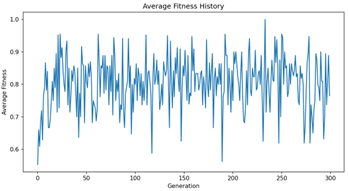
\includegraphics[width=\textwidth]{vt_only.png}
        % \caption{Subfigure 1}
        % \label{fig:sub1}
    \end{subfigure}
    % \hfill
    \begin{subfigure}[b]{0.05\textwidth}
        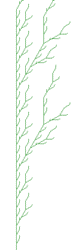
\includegraphics[width=\textwidth]{vt_only_dr.png}
        % \caption{Subfigure 2}
        % \label{fig:sub2}
    \end{subfigure}
    \vspace{0.5cm}
    \caption{$w_{vt}, w_{bs}, w_{s}, w_{pha}, w_{bp} = 100, 0, 0, 0, 0$}
    \label{fig:subfigures}
\end{figure}

\subsubsection{Bilateral Symmetry}
\begin{figure}[H]
    \centering
    \begin{subfigure}[b]{0.3\textwidth}
        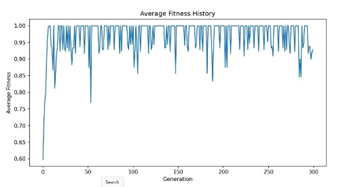
\includegraphics[width=\textwidth]{Sym_only_oa.png}
        % \caption{Subfigure 1}
        % \label{fig:sub1}
    \end{subfigure}
    % \hfill
    \begin{subfigure}[b]{0.1\textwidth}
        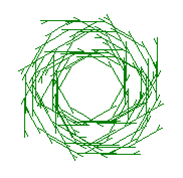
\includegraphics[width=\textwidth]{symm_only_dr.png}
        % \caption{Subfigure 2}
        % \label{fig:sub2}
    \end{subfigure}
    \begin{subfigure}[b]{0.1\textwidth}
        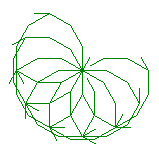
\includegraphics[width=\textwidth]{symm_only_dr2.png}
        % \caption{Subfigure 2}
        % \label{fig:sub2}
    \end{subfigure}
    \vspace{0.5cm}
    \caption{$w_{vt}, w_{bs}, w_{s}, w_{pha}, w_{bp} = 0, 100, 0, 0, 0$}
    \label{fig:subfigures}
\end{figure}

\subsubsection{Photon Gathering Ability}
\begin{figure}[H]
    \centering
    \begin{subfigure}[b]{0.3\textwidth}
        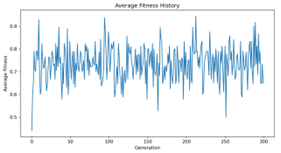
\includegraphics[width=\textwidth]{pg_only.png}
        % \caption{Subfigure 1}
        % \label{fig:sub1}
    \end{subfigure}
    % \hfill
    \begin{subfigure}[b]{0.1\textwidth}
        
\includegraphics[width=\textwidth]{pg_only_dr.png}
        % \caption{Subfigure 2}
        % \label{fig:sub2}
    \end{subfigure}

    \vspace{0.5cm}
    \caption{$w_{vt}, w_{bs}, w_{s}, w_{pha}, w_{bp} = 0, 0, 0, 100, 0$}
    \label{fig:subfigures}
\end{figure}

\subsubsection{Stability}
\begin{figure}[H]
    \centering
    \begin{subfigure}[b]{0.3\textwidth}
        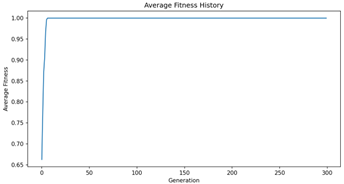
\includegraphics[width=\textwidth]{s_only.png}
        % \caption{Subfigure 1}
        % \label{fig:sub1}
    \end{subfigure}
    % \hfill
    \begin{subfigure}[b]{0.1\textwidth}
        
\includegraphics[width=\textwidth]{s_only_dr.png}
        % \caption{Subfigure 2}
        % \label{fig:sub2}
    \end{subfigure}

    \vspace{0.5cm}
    \caption{$w_{vt}, w_{bs}, w_{s}, w_{pha}, w_{bp} = 0, 0, 100, 0, 0$}
    \label{fig:subfigures}
\end{figure}

\subsubsection{Braching Proliferation}
\begin{figure}[H]
    \centering
    \begin{subfigure}[b]{0.3\textwidth}
        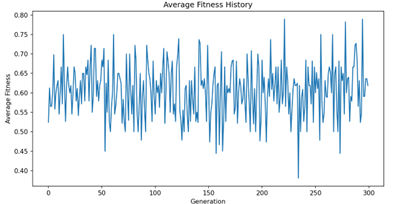
\includegraphics[width=\textwidth]{bp_only.png}
        % \caption{Subfigure 1}
        % \label{fig:sub1}
    \end{subfigure}
    % \hfill
    \begin{subfigure}[b]{0.1\textwidth}
        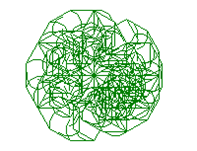
\includegraphics[width=\textwidth]{bp_only_dr.png}
        % \caption{Subfigure 2}
        % \label{fig:sub2}
    \end{subfigure}

    \vspace{0.5cm}
    \caption{$w_{vt}, w_{bs}, w_{s}, w_{pha}, w_{bp} = 0, 0, 100, 0, 0$}
    \label{fig:subfigures}
\end{figure}



\subsection{Block Mutation vs Symbol Mutation}

We implemented our system using both block mutation and symbol mutation. Figure~\ref{fig:mutation_comparison} and Figure~\ref{fig:mutation_comparison1}shows the comparison between the two mutation methods.

\begin{figure}[H]
    \centering
    \begin{subfigure}[b]{0.3\textwidth}
        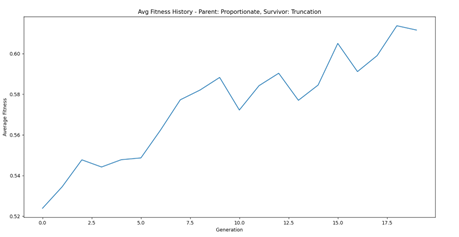
\includegraphics[width=\textwidth]{block1.png}
        % \caption{Subfigure 1}
        % \label{fig:sub1}
    \end{subfigure}
    % \hfill
    \begin{subfigure}[b]{0.1\textwidth}
        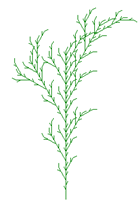
\includegraphics[width=\textwidth]{tree_block2.png}
        % \caption{Subfigure 2}
        % \label{fig:sub2}
    \end{subfigure}

    \vspace{0.5cm}
    \caption{$w_{vt}, w_{bs}, w_{s}, w_{pha}, w_{bp} = 100, 90, 40, 0, 80$}
    \label{fig:mutation_comparison}
\end{figure}

\begin{figure}[H]
    \centering
    \begin{subfigure}[b]{0.3\textwidth}
        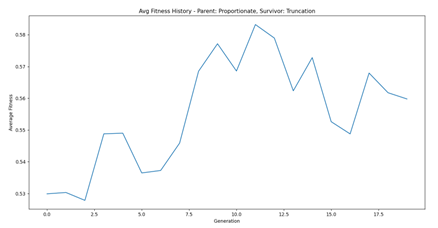
\includegraphics[width=\textwidth]{symbol.png}
        % \caption{Subfigure 1}
        % \label{fig:sub1}
    \end{subfigure}
    % \hfill
    \begin{subfigure}[b]{0.1\textwidth}
        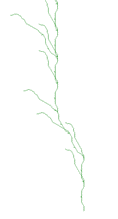
\includegraphics[width=\textwidth]{tree_sym.png}
        % \caption{Subfigure 2}
        % \label{fig:sub2}
    \end{subfigure}

    \vspace{0.5cm}
    \caption{$w_{vt}, w_{bs}, w_{s}, w_{pha}, w_{bp} = 100, 90, 40, 0, 80$}
    \label{fig:mutation_comparison1}
\end{figure}


We can observe from the figures that when we implemented the system with block mutation, it yielded better results compared to symbol mutation. This can be attributed to the fact that block mutation replaces a block of symbols rather than just a single symbol, allowing for larger-scale changes in the chromosome, which makes the population more diverse.


\subsection{Survivor Rank Based vs Survivor Truncation}

\begin{figure}[H]
    \centering
    \begin{subfigure}[b]{0.3\textwidth}
        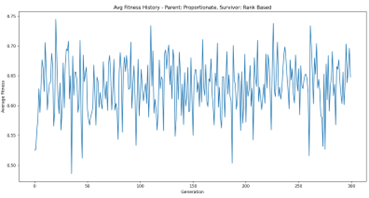
\includegraphics[width=\textwidth]{image2.png}
        % \caption{Subfigure 1}
        % \label{fig:sub1}
    \end{subfigure}
    % \hfill
    \begin{subfigure}[b]{0.1\textwidth}
        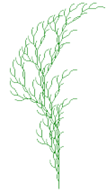
\includegraphics[width=\textwidth]{img2.png}
        % \caption{Subfigure 2}
        % \label{fig:sub2}
    \end{subfigure}

    \vspace{0.5cm}
    \caption{$w_{vt}, w_{bs}, w_{s}, w_{pha}, w_{bp} = 100, 90, 40, 0, 80$}
    \label{fig:mutation_comparison}
\end{figure}

\begin{figure}[H]
    \centering
    \begin{subfigure}[b]{0.3\textwidth}
        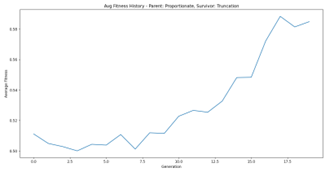
\includegraphics[width=\textwidth]{image1.png}
        % \caption{Subfigure 1}
        % \label{fig:sub1}
    \end{subfigure}
    % \hfill
    \begin{subfigure}[b]{0.1\textwidth}
        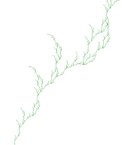
\includegraphics[width=\textwidth]{image.png}
        % \caption{Subfigure 2}
        % \label{fig:sub2}
    \end{subfigure}

    \vspace{0.5cm}
    \caption{$w_{vt}, w_{bs}, w_{s}, w_{pha}, w_{bp} = 100, 90, 40, 0, 80$}
    \label{fig:mutation_comparison}
\end{figure}

Implementing truncation in our system posed challenges, notably in the considerable time required for figure generation due to the significant increase in string length. Unlike truncation, this issue was not observed with the rank-based or any other survivor scheme. Due to limitations in computational resources, we could only implement truncation for 20 generations, compared to 300 generations in the case of rank-based selection. Despite this limitation, the figures clearly demonstrate that truncation outperforms rank-based selection by consistently selecting the fittest individuals, thus ensuring a higher overall performance.

\subsection{Parent Fitness Proportion vs Parent Tournament Selection}

\begin{figure}[H]
    \centering
    \begin{subfigure}[b]{0.3\textwidth}
        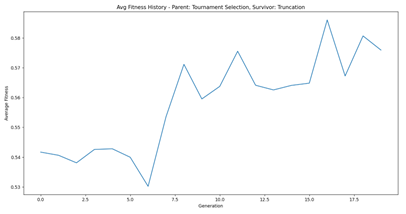
\includegraphics[width=\textwidth]{image3.png}
        % \caption{Subfigure 1}
        % \label{fig:sub1}
    \end{subfigure}
    % \hfill
    \begin{subfigure}[b]{0.1\textwidth}
        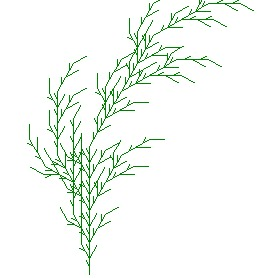
\includegraphics[width=\textwidth]{image6.png}
        % \caption{Subfigure 2}
        % \label{fig:sub2}
    \end{subfigure}

    \vspace{0.5cm}
    \caption{$w_{vt}, w_{bs}, w_{s}, w_{pha}, w_{bp} = 100, 90, 40, 0, 80$}
    \label{fig:mutation_comparison}
\end{figure}

\begin{figure}[H]
    \centering
    \begin{subfigure}[b]{0.3\textwidth}
        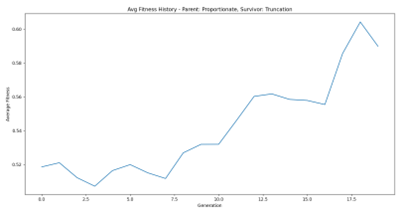
\includegraphics[width=\textwidth]{image5.png}
        % \caption{Subfigure 1}
        % \label{fig:sub1}
    \end{subfigure}
    % \hfill
    \begin{subfigure}[b]{0.1\textwidth}
        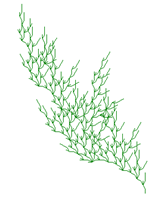
\includegraphics[width=\textwidth]{image7.png}
        % \caption{Subfigure 2}
        % \label{fig:sub2}
    \end{subfigure}

    \vspace{0.5cm}
    \caption{$w_{vt}, w_{bs}, w_{s}, w_{pha}, w_{bp} = 100, 90, 40, 0, 80$}
    \label{fig:mutation_comparison}
\end{figure}

In our system, we employed various parent selection schemes. However, when comparing tournament selection with fitness proportionate selection, the latter outperformed. This is because fitness proportionate selection consistently emphasizes choosing individuals based on their fitness, leading to a more directed evolutionary process. Conversely, tournament selection introduces randomness, potentially leading to suboptimal parent choices and slower convergence towards optimal solutions.


